\documentclass[12,french]{report}
\usepackage{geometry}
\geometry{vmargin=3cm, hmargin=3cm}
\usepackage[T1]{fontenc}
\usepackage[utf8]{inputenc}
\usepackage[french]{babel}
\usepackage{graphicx}
\usepackage{amsmath}
\usepackage{amssymb}
\usepackage{sectsty}
\usepackage{authblk}
\usepackage{algpseudocode}
\usepackage{algorithm}
\usepackage{xspace}
\usepackage{mathtools}
\usepackage{mathrsfs}
\usepackage{enumitem}
\usepackage{titlesec}
\usepackage{hyperref}
\usepackage{xcolor}
\usepackage[justification=centering]{caption}
\usepackage{float}
\usepackage{tabto}

\usepackage{listings}
\usepackage{cleveref}

\renewcommand{\lstlistingname}{Code}
%\renewcommand{\figurename}{Fig.}

\lstdefinestyle{chstyle}{%
backgroundcolor=\color{gray!12},
basicstyle=\ttfamily\small,
showstringspaces=false,
numbers=left}

%\AddThinSpaceBeforeFootnotes
%\FrenchFootnotes

\titleformat{\chapter}[hang]{\bf\Huge}{\thechapter.}{2pc}{}
\titlespacing*{\chapter}{10pt}{0pt}{40pt}[0pt]
\newcommand{\HRule}{\rule{\linewidth}{0.5mm}}

\providecommand{\keywords}[1]{\textbf{\textit{Keywords:}} #1}
\bibliographystyle{apalike}

\usepackage{hyperref}

\begin{document}
\hypersetup{pdfborder=0 0 0}

\begin{titlepage}

\begin{center}
	\vspace*{\stretch{1}}
	\textsc{{\LARGE Institut national des sciences appliquées de Rouen} \\ 			\vspace{6mm} {\Large INSA de Rouen}} \\
	\vspace{5mm}
	
\includegraphics[width=0.4\textwidth]{./Images/insa}\\[1.0 cm]

	\textsc{\Large Mini-projet COO - GM3}\\[0.6cm]

	% Title
	\HRule \\[0.5cm]
	{ \Huge \bfseries Réalisation d'un jeu de dames en Java}\\[0.2cm]
	\HRule \\[0.75cm]

	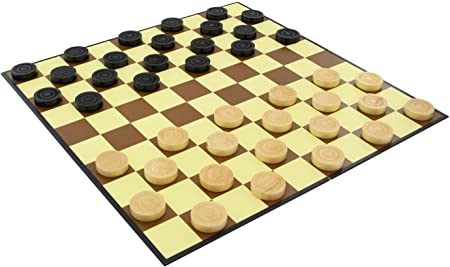
\includegraphics[width=0.7\textwidth]{./Images/Page_de_garde}\\[0.9 cm]

	% Author and supervisor
	\begin{minipage}{0.4\textwidth}
		\begin{flushleft} \large
			\emph{Auteurs:}\\
			Thibaut \textsc{André-Gallis} \\
			{\small\href{mailto:thibaut.andregallis@insa-rouen.fr}{thibaut.andregallis@insa-rouen.fr}} \\
			Kévin \textsc{Gatel} \\
			{\small\href{mailto:kevin.gatel@insa-rouen.fr}{kevin.gatel@insa-				rouen.fr}}
		\end{flushleft}
	\end{minipage}
	\begin{minipage}{0.4\textwidth}
		\begin{flushright} \large
			\emph{Enseignants:} \\
			Mathieu \textsc{Bourgais} \\
			{\small\href{mailto:mathieu.bourgais@insa-rouen.fr}								{mathieu.bourgais@insa-rouen.fr}}\\
			Habib \textsc{Abdulrab} \\
			{\small\href{mailto:habib.abdulrab@insa-rouen.fr}{habib.abdulrab@insa-rouen.fr}}
		\end{flushright}
	\end{minipage}
	\vspace*{\stretch{1}}

	\vfill
	{\large 23 Mai 2021}
\end{center}
\end{titlepage}

\tableofcontents

%\listoffigures

\renewcommand{\chaptername}{}
\chapter*{Introduction}

Le mini-projet que nous avons choisi est la réalisation du jeu de dames en Java.\\

Le jeu de dames est un célèbre jeu de réflexion joué à deux inventé pour la première fois en Egypte antique vers -1500 avant J-C.
Pour la version classique, le jeu de dames est composé d'un damier de 10 cases sur 10 cases de deux couleurs alternées et d'une vingtaine de pions par joueur disposés les uns en face des autres. Il existe également des variantes de ce jeu qui utilisent des damiers de 64 cases (8 sur 8) et 144 cases (12 par 12). 
Le but du jeu est alors de capturer ou d'immobiliser toutes les pièces du joueur adverse. \\

Le but de ce projet est d'utiliser habilement les concepts de la programmation objet, c'est-à-dire savoir écrire les différents diagrammes, maîtriser l'héritage entre les classes, le polymorphisme, la gestion des interfaces ou des classes arbitraires, etc...\\

Pour bien répondre au problème, nous allons d'abord regarder le \textbf{diagramme de cas} (Use-cases) et le \textbf{diagramme de classe} (UML) afin de comprendre l'organisation du code.\\

Ensuite, nous allons présenter et décrire le rôle de \textbf{chacune des classes} qui ont été nécessaires à la réalisation du projet.\\

Enfin, nous verrons \textbf{les différents problèmes} que nous avons pu rencontrer lors de la programmation du jeu.


\chapter{Les diagrammes}

\section{Use-cases}

\begin{figure}[H]
	\center
	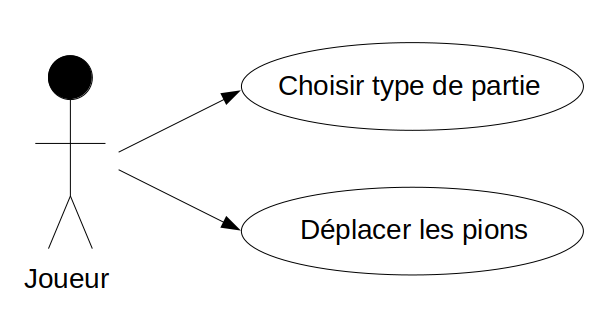
\includegraphics[width=0.7\textwidth]{./Images/Use-cases}
	\caption{Diagramme de cas pour le jeu de dames}
\end{figure}\vspace{0.2cm}

Les joueurs commencent par choisir la variante de leur choix pour jouer au jeu de dames. Ils ont le choix entre :

\begin{itemize}[label=\textbullet]
	\item Une partie rapide : damier 8 sur 8 où chaque joueur possède 16 pièces.
	\item Une partie classique : damier 10 sur 10 où chaque joueur possède 20 pièces.
	\item Une partie longue : damier 12 sur 12 où chaque joueur possède 24 pièces.
\end{itemize}\vspace{0.3cm}

Ils choisissent ensuite s'ils veulent ou non obliger le saut de pièce (dans la version classique le saut est obligatoire).\\

La partie se lance et les joueurs déplacent chacun leur tour une pièce de leur couleur jusqu'à ce que la partie se termine.


\section{UML}

\begin{figure}[H]
	\center
	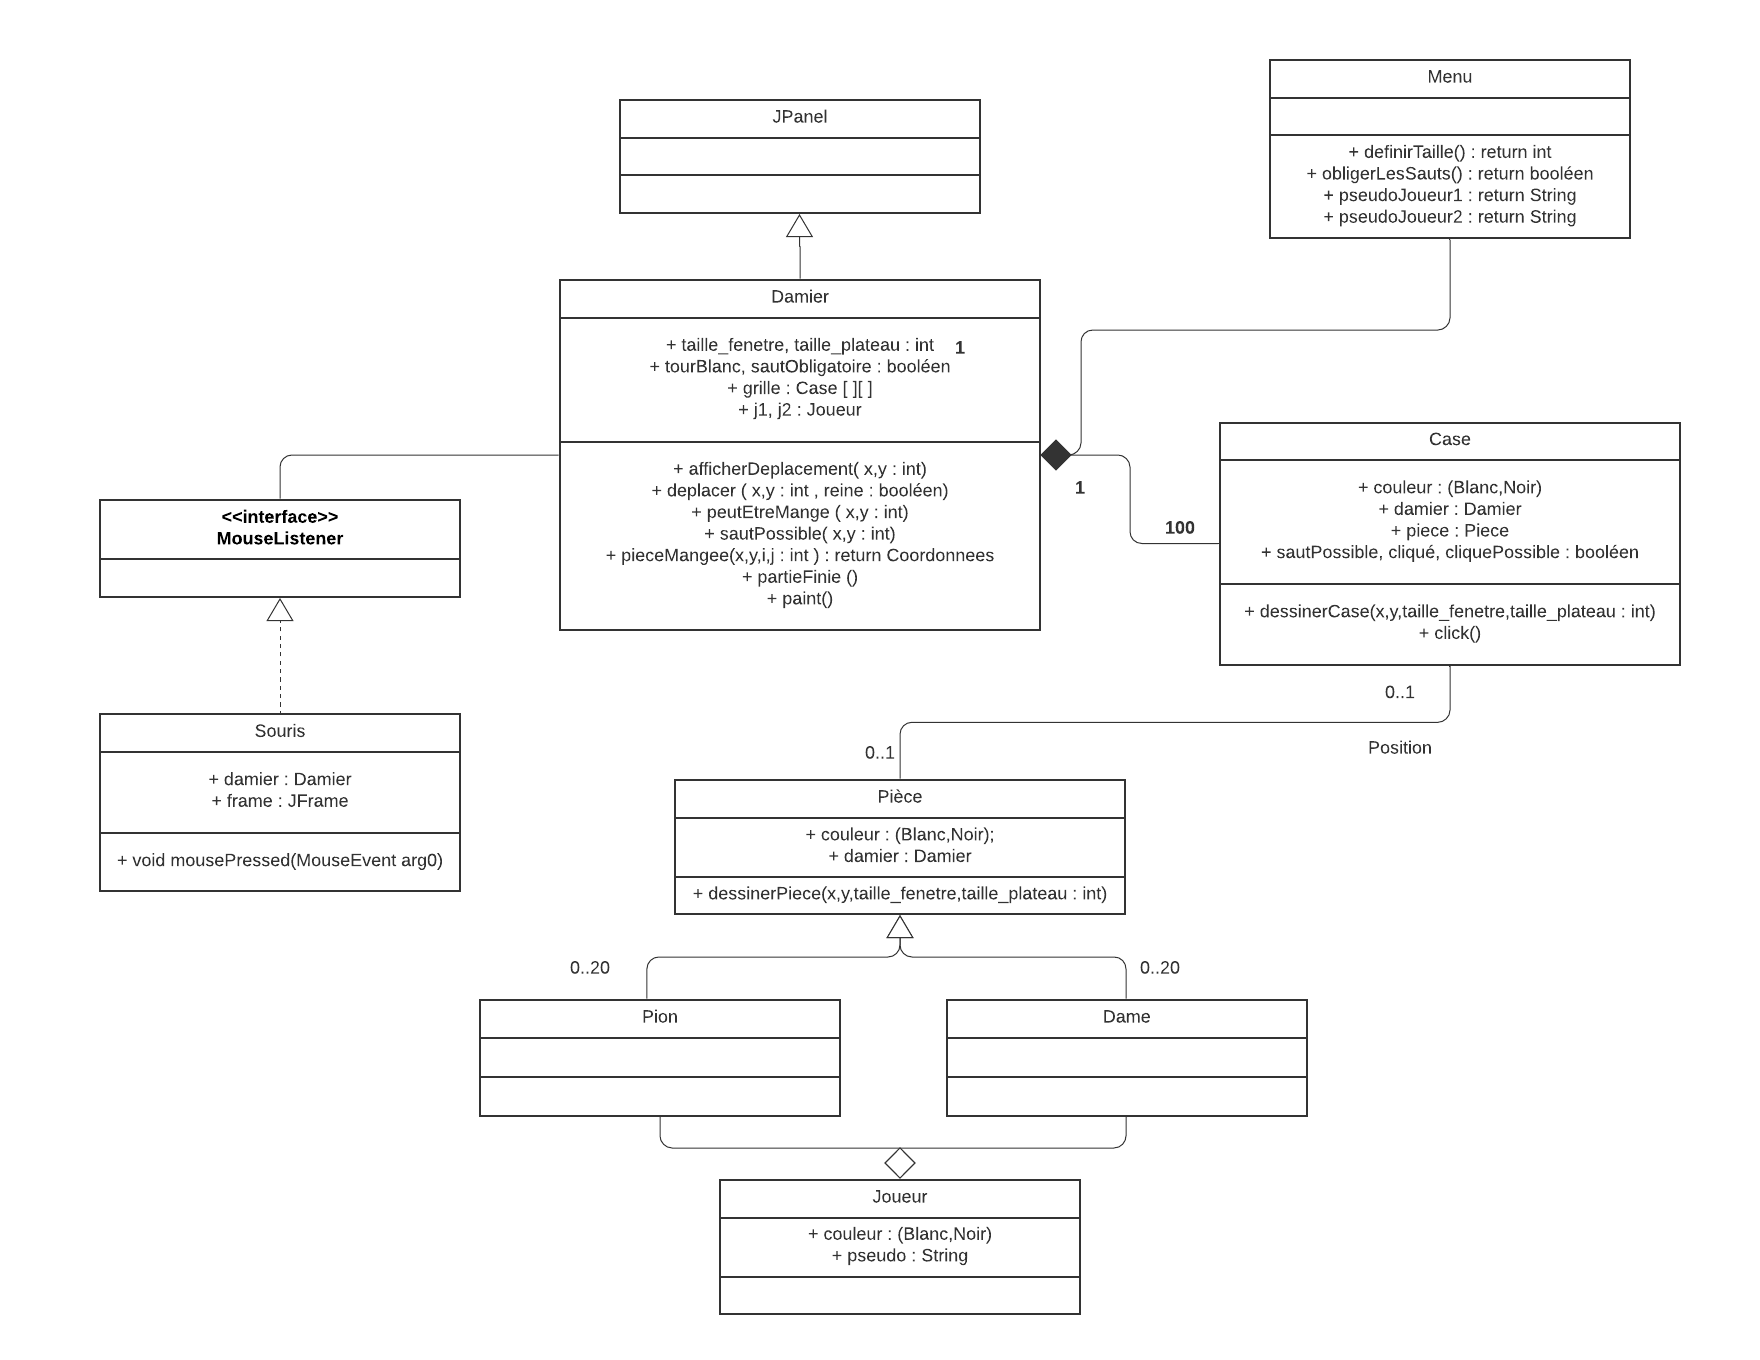
\includegraphics[width=1\textwidth]{./Images/UML}
	\caption{Diagramme de classe pour le jeu de dames}
\end{figure}\vspace{0.2cm}

La classe \textit{Menu.java} est la première classe utilisée lors du lancement du programme. On définit ici la taille du plateau, on demande aux joueurs s'ils veulent ou non obliger les sauts et on récupère leur pseudo respectif.\\

La classe \textit{Damier.java} est la classe centrale du projet. Elle permet le déplacement des pièces, l'affichage du damier et la gestion des cases. Grâce à la classe \textit{JPanel}, elle hérite de la méthode prédéfinie \textit{void paint(Graphics g)} qu'on a modifié en utilisant les méthodes \textit{void dessinerPiece()} et \textit{void dessinerCase()} et permet ainsi l'affichage du plateau.\\

La méthode \textit{void afficherDeplacement(x,y : int)} va colorier les cases disponibles d'une certaine couleur pour le déplacement d'une pièce de coordonnées (x,y). On coloriera en bleu un déplacement sans saut de pièce et en rose pour un déplacement avec saut de pièce.\\

La méthode \textit{void déplacer(x,y : int)} va permettre ou non le déplacement d'un pion déjà sélectionné sur une case de coordonnées (x,y). Le déplacement sera autorisé si la case a été colorée en bleu ou en rose. Si la case (x,y) est rose, on utilise la méthode \textit{boolean sautPossible} pour savoir s'il peut continuer à jouer, à savoir s'il peut sauter des pièces, le tour du joueur sera alors inchangé.

A chaque saut, on utilise la méthode \textit{Coordonnees pieceMangee(x,y,i,j : int)} qui retourne les coordonnées de la pièce mangée, pour ensuite l'enlever du plateau.\\

A la fin du tour, on utilise la méthode \textit{boolean peutEtreMange(x,y : int)} sur chaque pièce du joueur. S'il s'avère qu'une pièce peut être mangé au tour d'après, si l'option \textit{sautObligatoire} a été choisie par les joueurs en début de partie, tout déplacement du joueur suivant n'étant pas un saut est bloqué, un message d'erreur est affiché si nécessaire.\\

La méthode \textit{boolean partieFinie()} retourne vrai si un joueur ne possède plus de pion ou ne peut plus en déplacer. La partie se termine et un message affiche le vainqueur du jeu.\\

La classe \textit{Souris.java} va permettre aux joueurs de déplacer leur pièce grâce au clique de la souris. En effet, elle est issue de l'interface \textit{MouseListener} qui comprend de nombreuses méthodes prédéfinies. En modifiant la méthode \textit{void mousePressed(MouseEvent arg0)} on est capable de récupérer l'endroit où le joueur clique pour ensuite effectuer des actions sur le damier placé en attribut.


\chapter{Les classes}

\section{Case}

La classe \textit{Case} possède une couleur et une pièce. Pour les cases ne contenant aucune pièce, on fixera l'attribut \textit{piece} en \textit{null}. Il est alors impératif de vérifier à chaque fois si la pièce d'une case existe ($\neq$ \textit{null}) avant de demander la couleur d'un pion ou d'une reine.


\section{Coordonnes}

La classe \textit{Coordonnees} ne possède aucune méthode. Elle a été créée dans le seul but de concevoir une fonction (présente dans la classe \textit{Damier}) qui retournerait les coordonnées d'une pièce mangée.

\section{Couleur}

La classe \textit{Couleur} est une classe énumération. Elle contient uniquement les deux couleurs nécessaires : Blanc et Noir.

\section{Damier}

La classe \textit{Damier} est la classe principale du programme. Elle regroupe l'ensemble des procédures de déplacement et d'affichage du jeu. Grâce à la classe \textit{JPanel}, elle hérite de la procédure \textit{paint()} qui va permettre ainsi en la redéfinissant d'afficher le damier et ses pièces. Ses attributs comme sa taille ou encore son booléen \textit{sautObligatoire} est fixé par l'utilisateur au début du jeu. Pour manipuler les pièces, il possède un tableau deux dimensions de \textit{Case} permettant ainsi de connaître l'ensemble du plateau à chaque instant.

\section{Joueur}

La classe \textit{Joueur} contient en attribut le pseudo (fixé dans la classe \textit{Menu}) et la couleur du joueur. Le premier joueur a la couleur blanche, le second la couleur noire.

\section{Lanceur}

La classe \textit{Lanceur} est la classe \textit{Main} de notre projet. Elle permet de lancer le jeu. Elle lance d'abord le menu puis affiche le damier et les pions afin de débuter une partie.

\section{Menu}

La classe \textit{Menu} demande aux joueurs le type de partie qu'ils veulent jouer afin de déterminer la taille du plateau. Elle demande également si les joueurs veulent jouer avec l'option "Saut Obligatoire". Les joueurs choisissent également leur pseudo grâce à cette classe. Cette classe sert uniquement au démarrage de la partie, avant même que le plateau soit affiché.

\section{Piece}

La classe \textit{Piece} est la sous-classe de tous les pions et reines du plateau. Elle contient en attribut la couleur de la pièce et contient une seule méthode qui permet de dessiner la pièce selon sa couleur et selon s'il s'agit d'un pion ou d'une reine. Elle appartient forcément à une case c'est pour cette raison qu'il n'y a pas d'attribut \textit{Coordonnees}.

\section{Pion}

La classe \textit{Pion} hérite de la classe \textit{Piece}. Elle ne contient pas plus de méthode ni d'attribut.

\section{Reine}

La classe \textit{Reine} hérite de la classe \textit{Piece}. Identiquement à la classe \textit{Pion}, elle ne contient pas plus de méthode ni d'attribut.
\section{Souris}

La classe \textit{Souris} est une des plus importantes du projet. En effet, elle permet aux joueurs de pouvoir jouer avec la souris. C'est elle qui va gérer l'intéraction homme-machine. Grâce à l'interface \textit{MouseListener} déjà prédéfinie, elle a accès a plusieurs méthodes dont \textit{void mousePressed(MouseEvent arg0)} qui écoute chaque pression d'un bouton sur la souris. Avec les fonctions \textit{getX} et \textit{getY} on récupère les coordonnées où le joueur clique dans la fenêtre. Ces coordonnées sont ensuite filtrés puis selon la case, la pièce indiquée des décisions sont prises.

\chapter{Problèmes rencontrés}

\section{Affichage}

L'affichage du damier et des pièces fut notre première mission lors du codage du jeu.
Il nous semblait primordial d'observer directement ce que l'on allait coder afin de remarquer les éventuelles erreurs ou oublis.\\

Nous avons donc utiliser l'environnement \textit{swing} du paquet \textit{javax} afin de pouvoir afficher notre plateau. L'environnement étant tout nouveau pour nous, il nous a fallu beaucoup de temps afin de comprendre comment il s'utilise. Avec \textit{JFrame} nous pouvions ouvrir une nouvelle fenêtre et la renommer "Jeu de dames", puis avec l'héritage de la classe \textit{JPanel} la méthode \textit{paint} pouvait dessiner ce que l'on souhaitait sur la fenêtre en question.\\

Au départ nous avons fait cet affichage sur un plateau d'une taille fixée 10 par 10. Puis nous voulions étendre cet affichage pour n'importe quelle taille donnée, il nous a fallu alors introduire une échelle TAILLE/taille et comprendre comment bien l'utiliser (TAILLE correspond à la taille de la fenêtre et taille correspond à la taille du damier). Cette échelle nous a permis notamment de centrer les pièces dans chaque case du damier. Ainsi, nous pouvons fabriquer un damier de la taille que l'on souhaite (réglable dans la classe \textit{Lanceur}).\\

Malheureusement, un mini problème persiste encore au niveau de l'affichage. Il s'agit d'une barre noire verticale à droite de la fenêtre qui apparaît uniquement au lancement d'une partie. Il était pour nous impossible de régler ce léger problème ne comprenant pas l'origine de l'existence. Après réflexion, nous avons compris qu'il s'agissait d'un problème de paquet et non de codage, nous avons donc abandonné la recherche de la solution. Ce problème apparaissant en moyenne 2 fois sur 3 lancement de partie disparaît au premier clique de la souris, ce qui est au final peu dérangeant.
 
\section{Ecoute de la souris}

L'écoute de la souris nous a également posé de nombreux problèmes. La classe \textit{MouseListener} étant également nouveau pour nous, la comprendre était pas chose facile au début du projet. En effet, nous voulions au départ écouter chaque case afin de récupérer la case cliquée directement. Nous avons alors remarqué des anomalies sur le comportement des méthodes de la classe. Nous avons donc décidé d'écouter le plateau entier puis de filtrer les coordonnées de l'endroit cliqué afin de déterminer la case correspondante.


\chapter*{Conclusion}
\addcontentsline{toc}{chapter}{Conclusion}


\end{document}
